	\chapter{LANDASAN TEORI}
	Bab ini akan membahas mengenai dasar teori dan literatur yang menjadi dasar pengerjaan tugas akhir ini. Pada subbab 2.1 membahas mengenai deskripsi permasalahan. Pada subbab 2.2 membahas mengenai contoh permasalahan. Pada subbab 2.3 membahas mengenai definisi umum yang digunakan dalam memecahkan permasalahan ini. Pada subbab 2.4 membahas mengenai penyelesaian masalah secara lengkap.
	\section{Deskripsi Permasalahan}
	\label{chapter:dasar-teori}
	Permasalahan yang diangkat dalam tugas akhir ini diangkat dari suatu permasalahan yang terdapat pada suatu situs penilaian daring atau \textit{online judge} SPOJ yaitu \textit{The Bytelandian Cryptographer (Act IV)} dengan nomer soal 20 dengan kode soal CRYPTO4. Deskripsi soal yang asli menggunakan bahasa Inggris dapat dilihat pada \ref{fig:crypto4_def}.\cite{piwakowski_crypto4_2004}
	
	
	 Permasalahan pada The Bytelandian Cryptographer (Act IV) diberikana pesan dengan panjang $N$ huruf, huruf yang digunakan adalah huruf kapital latin dari A sampai dengan Z, yang dapat ditafsirkan menjadi bilangan bulat dari 0 sampai dengan 25. Diberikan kunci untuk mentransmisikan pesan yang diketahui oleh kedua belah pihak yang terdiri dari $M$ bilangan bulat. Dengan menggunakan kunci yang ada bahwa pada index ke $i$ dari pesan pada index $x_i$ akan di enkripsikan ke dalam bentuk index ke $i$ dari pesan hasil enskripsi $y$, yang mengikuti aturan
	 $$y_i=x_i+k_{1+(i-1)mod M} mod 26 $$
	 
	 
	 Diketahui \textit{plain text} dan \textit{ciphertext} yang diberikan hanya berupa potongan-potongan dari kedua pesan tersebut. Dicari bagaimana menkonstruksi ulang pesan yang telah didapat sehingga bisa membentuk \textit{plain text} yang asli dari pesan yang telah didapatkan sebanyak-banyaknya.
	\begin{figure}[H]
		\centering
		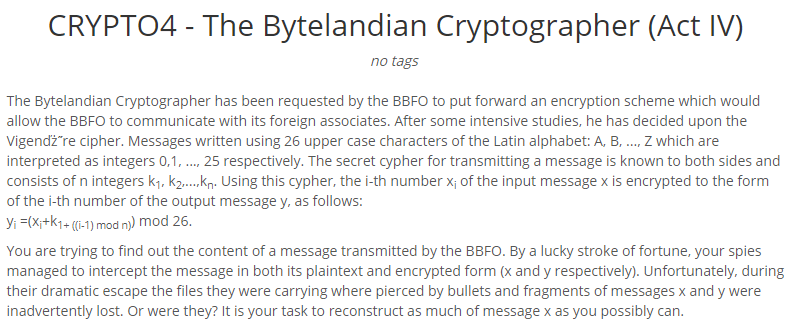
\includegraphics[scale=0.5]{images/bab2/crypto_def.png}
		\caption{Deskripsi Permasalahan pada SPOJ \textit{The Bytelandian Cryptographer (Act IV)}}
		\label{fig:crypto4_def}
	\end{figure}
	
	
	Format masukan pada baris pertama diberikan $T$ ujicoba kasus. Pada baris selanjutnya diberikan $M$ batas atas panjang kunci. Pada baris selanjutnya diberikan \textit{plain text}. Pada baris selanjutnya di berikan \textit{ciphertext}, \textit{plain text} dan \textit{ciphertext} menggunakan karakter A sampai dengan Z yang dapat ditafsirkan kedalam bilangan bulat 0 sampai dengan 25 dan '*'(sebagai karakter yang hilang).
	
	
	Format keluaran yang dihasilkan adalah 1 baris yang mengandung \textit{plain text} dan '*' apabila nilai dari karakter tersebut tidak dapat ditentukan.
	
	
	Deskripsi mengenai Format masukan dan keluaran beserta dengan contohnya dalam bahasa Inggris dapat lihat pada gambar \ref{fig:crypto4_io}
	\begin{figure}[H]
		\centering
		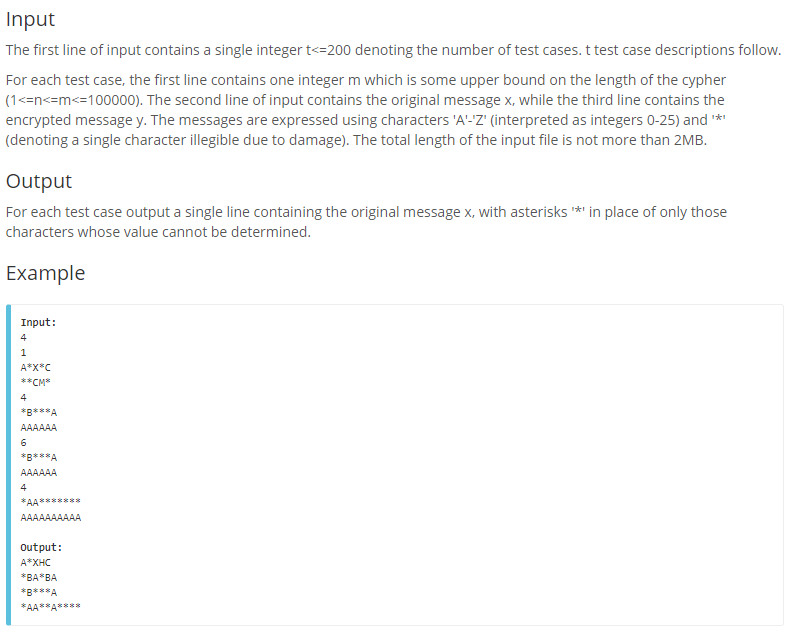
\includegraphics[scale=0.5]{images/bab2/crypto_io.png}
		\caption{Deskripsi Format Masukan dan Keluaran pada SPOJ \textit{The Bytelandian Cryptographer (Act IV)}}
		\label{fig:crypto4_io}
	\end{figure}
	
	
	Batasan permasalahan \textit{The Bytelandian Cryptographer (Act IV)} adalah sebagai berikut:
	\begin{enumerate}
		\item $T<=200$
		\item $1<=M<=n<=100,000$
		\item Panjang \textit{input file} tidak melebihi dari 2MB.
		\item Lingkungan penilaian Intel Pentium G860 3GHz.
		\item Batas Waktu: <=17 detik
		\item Batas Sumber Code : 50000B
		\item Batas Memory : 1536 MB.                 
	\end{enumerate}\cite{piwakowski_crypto4_2004}

	\section{Contoh Kasus Permasalahan}
	Contoh 1.Diketahui $M$ bernilai 1 yang menunjukkan batas atas dari panjang kunci. Diketahui \plaintext adalah A*X*C dan \ciphertext adalah **CM*. Indek akan dihitung mulai dari 0. 
	\begin{table}[H]
	 	\centering
	 	\begin{tabular}{|c|c|c|c|c|c|c|}\hline
	 	\textit{plain text}&A&*&X&*&C\\ \hline
	 	\textit{ciphertext}&*&*&C&M&*\\ \hline
	 	\end{tabular}
	 	\caption{Contoh 1}
	 	\label{tab:contoh1}
	\end{table}
	 Dari table \ref{tab:contoh1} dapat dilihat bahwa index 0 tidak perlu di rubah lagi. index 1 tidak di ketahui dua duanya maka tidak bisa di cari. index 2 sudah ada jadi tidak usah di cari lagi. Index 3 di ketahui \textit{ciphertext} dan diketahui bahwa batas atasnya 1 maka kita sudah pasti bisa memastikan bahwa panjang kucinya adalah 1, karena batas atas sama dengan batas minimum untuk membuat suatu teknik subtitusi \textit{cipher}, selain itu juga di ketahui bahwa pada index 2 selisih antara \textit{plaintext} dan \textit{ciphertext} adalah . Maka dapat diambil suatu kesimpulan bahwa \textit{plain text} index ke 3 adalah H. Index 4 sudah di ketahui juga. 
	 
	 
	 Contoh 2. Diketahui bahwa $M$ bernilai 4 yang menunjukkan batas atas dari panjang kunci. Diketahui\plaintext adalah *B***A dan \ciphertext adalah AAAAAA. Indek akan dihitung mulai dari 0. 
	 \begin{table}[H]
	 	\centering
	 	\begin{tabular}{|c|c|c|c|c|c|c|c|}\hline
	 	\textit{plain text}&*&B&*&*&*&A\\ \hline
	 	\textit{ciphertext}&A&A&A&A&A&A\\ \hline
	 	\end{tabular}
	 	\caption{Contoh 2}
	 	\label{tab:contoh2}
	\end{table}
	Dari table \ref{tab:contoh2} dapat diketahui pada indeks 1 selisih antara \plaintext dan \ciphertext adalah 25 dan indeks 5 selisih antara \plaintext dan \ciphertext adalah 0. Selanjutnya disebut sebagai indeks yang diketahui. Kemudian mencoba untuk menebak panjang kuncinya dari 1 sampai dengan 4. Pertama-tama mencoba panjang kuncinya adalah 1, ternyata hal itu tidak mungkin kepada indeks yang diketahui apabila dimodulokan dengan 1 hasilnya 1 semua, sehingga tidak mungkin menggunakan panjang kunci 1. Hal itupun juga berlaku apabila panjang kuncinya dimodulokan 2 hasilnya salah, karena indeks yang diketahui di modulokan 2 juga hasilnya 1 semua. Maka kunci yang panjangnya 4 pun juga tidak benar karena 2 sudah salah maka kelipatannya pun pasti salah. Maka yang tersisa hanya tinggal panjang kunci 3, apabila dari indeks yang diketahui dimodulokan dengan 3 ternyata hasilnya indeks 1 dimodulo 3 hasilnya 1 dan indeks 5 dimodulo 3 hasilnya 2. Sehingga dapat disimpulkan bahwa panjang kunci 3 adalah benar. \textit{Plain text} yang terbentuk adalah *BA*BA, karena indeks ke 2 dapat diambilkan dari indeks ke 5 yaitu  selisihnya 0 dari \textit{ciphertext}. Karena  $5\%3=2$, sedangkan indeks ke 4 dapat diambilkan dari indeks 1 karena $ 4\%3=1 $ yang selisihnya 25. 
	
	
	Contoh 3. Diketahui bahwa $M$ bernilai 4 yang menunjukkan batas atas dari panjang kunci. Diketahui \plaintext adalah *AA******* dan \ciphertext adalah AAAAAAAAAA. Indek akan dihitung mulai dari 0.
	 \begin{table}[H]
	 	\centering
	 	\begin{tabular}{|c|c|c|c|c|c|c|c|c|c|c|}\hline
	 	\textit{plain text}&*&A&A&*&*&*&*&*&*&*\\ \hline
	 	\textit{ciphertext}&A&A&A&A&A&A&A&A&A&A\\ \hline
	 	\end{tabular}
	 	\caption{Contoh 3}
	 	\label{tab:contoh3}
	\end{table}
	
	\begin{table}[H]
		\centering
		\begin{tabular}{|c|c|c|c|c|c|c|c|c|c|c|}\hline
		\textit{plain text} awal&*&A&A&*&*&*&*&*&*&*\\ \hline
		Panjang kunci 1 &A&A&A&A&A&A&A&A&A&A\\ \hline
		Panjang kunci 2 &A&A&A&A&A&A&A&A&A&A\\ \hline
		Panjang kunci 3 &*&A&A&*&A&A&*&A&A&*\\ \hline
		Panjang kunci 4 &*&A&A&*&*&A&A&*&*&A\\ \hline
		Hasil Akhir     &*&A&A&*&*&A&*&*&*&*\\ \hline
		\end{tabular}
		\caption{Hasil dari Contoh 3}
		\label{tab:res_contoh_3}
	\end{table}
	Keempat panjang kunci tersebut benar terhadap pesan tersebut. Hasil keluaran yang diinginkan hanya 1 saja tetapi keempat-empatnya benar, oleh karena itu perlu dilakukan \textit{intersection} atau perpotongan dari himpunan keempat kunci tersebut. Perpotongan itu mengahasilkan {,A,A,,A,,,,,}. Terdapat bagian bagian yang kosong yang dapat  diisi dengan *. Sehingga hasil akhirnya dapat dilihat pada tabel \ref{tab:res_contoh_3} pada bagian hasil akhir.
	
	\section{Definisi Umum}
	Pada subbab ini membahas definisi-definisi yang digunakan sebagai dasar untuk memahami permasalahan ini dan pemecahannya.	
	\subsection{Polyalphabetic Cipher}
	\textit{Polyalphabetic Cipher }merupakan salah satu teknik untuk menenkripsi dengan menggunakan subtitusi huruf untuk menyubtitusikannya. Secara garis besar yang dimaksud dengan \textit{polyalphabetic cipher} memiliki 2 aturan dasar yang harus dipenuhi yaitu :
	\begin{enumerate}
		\item Memiliki satu set aturan subtitusi \textit{monoalphabetic cipher} yang digunakan.
		\item Sebuah kunci mengatur suatu aturan tertentu yang dipilih untuk mengatur transformasi yang dilakukan.
	\end{enumerate}
	Untuk memperjelas aturan diatas, dapat dilihat pada gambar \ref{fig:polyalphabeticalcipher}.
	\begin{figure}[H]
		\centering
		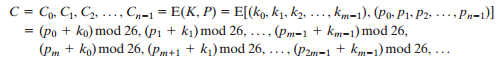
\includegraphics[scale=0.85]{images/bab2/poly.png}
		\caption{Aturan \textit{Polyalphabetical Cipher}}
		\label{fig:polyalphabeticalcipher}
	\end{figure}
	Salah satu turunan dari \textit{polyalphabetic cipher} adalah teknik \textit{Vigenere Cipher} yang menjadi dasar permasalahan yang diangkat dalam tugas akhir ini.\cite{stallings_computer_2015}
	
	\subsection{Ciphertext}
	\textit{Ciphertext} adalah suatu pesan / teks acak yang dihasilkan dari suatu algoritma kriptografi.\cite{william_crytography_2011}
	
	\subsection{Plaintext}
	\textit{Plaintext} Plaintext adalah data original sebagai inputan dari suatu metode enskripsi yang akan dilakukan.\cite{william_crytography_2011}
	
	\subsection{Secret Key}
	\textit{Secret Key} atau yang lebih dikenal dengan \textit{key} adalah suatu inputan dari algoritma enskripsi yang akan menentukan suatu transformasi dan subtitusi yang akan dilakukan oleh algoritma enskripsi.\cite{william_crytography_2011}
	
	 \subsection{Kasiski Examination}
	 \textit{Kasiski Examination} merupakan suatu teknik yang digunakan untuk mendeskripsikan secara paksa suatu \textit{ciphertext} yang menggunakan teknik subtitusi, baik itu \textit{polyalphabetical cipher} maupun \textit{monoalphabetical cipher}. Teknik menggunakan kelemahan yang ditimbulkan oleh teknik subtitusi itu sendiri, yaitu apabila suatu \textit{subtring} dari \plaintext dan \textit{subtring} dari suatu set kunci yang berulang terdapat yang berulang, maka dapat dipastikan untuk menebak panjang huruf / karakter kunci yang digunakan. Sebagai contoh dapat dilihat pada table \ref{tab:kasiski examination}.
	 \begin{table}[H]
		\centering
		\begin{tabular}   {|c|c|c|c|c|c|c|c|c|c|c|c|c|c|c|c|c|c|c|c|c|c|c|c|c|c|c|c|c|c|c|c|c|}\hline
		\textit{plain text}&c&r&y&p&t&o& &i&s& &s&h&o&r&t& &f&o&r& &c&r&y&p&t&o&g&r&a&p&h&y\\ \hline
		kunci&a&b&c&d&e&a&b&c&d&e&a&b&c&d&e&a&b&c&d&e&a&b&c&d&e&a&b&c&d&e&a&b\\ \hline
		\end{tabular}
		\caption{Contoh \textit{Kasiski Examintaion}}
		\label{tab:kasiski examination}
	\end{table}
	Dari table \ref{tab:kasiski examination} yang ada dapat disimpulakan bawah \plaintext "crypto" dan kunci "abcdea" berulang. Sehingga setidaknya dapat disimpulkan bahwa panjang kuncinya mungkin 4 karakter. \cite{noauthor_kasiski_nodate}. Hal ini yang menjadi dasar pengerjaan permasalahan yang diangkat dalam tugas akhir ini.
	\subsection{Intersection}
	\textit{Intersection} adalah himpunan A dan Himpunan B dimana ada bagian dari A juga merupakan bagian dari B. Sehingga dapat ditulis 
	$$A\cap{B=\{x:x\in A \textrm{ dan } x \in B \}}$$
	Sebagai contoh \textit{intersection} antara $\{1,2,3\}$ dan $\{1,4,5\}$ adalah $\{1\}$.\cite{devlin_joy_1993}
	
	\section{Penyelesaian Masalah The Bytelandian Cryptographer (Act IV)}
	\label{chapter:solving}
	Permasalahan \textit{The Bytelandian Cryptographer (Act IV)} dapat diselesaikan dengan menggunakan \textit{Kasiski Examination} dan \textit{Intersection}. Berikut ini tahapan-tahapan untuk menyeselsaikan masalah ini:
	\begin{enumerate}
	\item Menyimpan posisi indeks karakter, dimana pada indeks tersebut baik \ciphertext maupun \plaintext tidak bernilai '*', besertra menyimpan hasil perhitungan selisih antara \ciphertext dan \plaintext\cite{john_jones_spoj_2009}.
	\item Menyimpan posisi indeks, apabila /ciphertext diketahui dan \plaintext tidak diketahui. Untuk mengurangi \textit{running time} dari program\cite{john_jones_spoj_2009}.
	\item Mengiterasi panjang kunci dari $\frac{M}{2}+1<=N<=M$, alasannya dimulai dari $\frac{M}{2}+1$ tidak dari $1$ karena apabila suatu panjang kunci bernilai benar maka kelipatan dari panjang kunci itu pun juga pasti benar dan untuk mempersingkat waktu \textit{running time} yang seharusnya terjadi. Yang mendasari ini adalah dari table \ref{tab:contoh2} pada bagian 2.2. Pada bagian ini dilakukan untuk mencari panjang kunci yang benar dengan cara mengiterasi hasil yang diperoleh pada tahap 1 dimodulo dengan posisi iterasi yang dilakukan, apabila tidak terjadi konflik maka panjang kunci tersebut benar jika sebaliknya yang terjadi maka pnajang kunci tersebut tidak salah. Contohnya dapat dilihat pada contoh 2 pada bagian 2.2. Pada bagian ini memungkinkan bahwa bisa jadi lebih dari 1 panjang kunci yang bernilai benar. Contohnya seperti yang terjadi pada table \ref{tab:contoh3} pada bagian 2.2. 
	\item Melakukan \textit{intersection} terhadap himpunan dari kunci yang telah di hasilkan\cite{john_jones_spoj_2009}. \textit{intersection} yang dilakukan berada didalam perulangan panjang kunci pada waktu generate setiap karakter yang terdapat dalam penyimpanan tahap 2 pada panjang kunci tersebut dengan ketentuan:
	\begin{enumerate}
	\item Panjang kunci harus benar
	\item Apabila terdapat indeks yang tidak dapat dipastikan isinya maka posisinya harus di buang dari penyimpanan dan hasilnya pasti '*'
	\end{enumerate}
	\end{enumerate}
	Sehingga untuk setiap \textit{textcase} kompleksitasnya 
	$$\mathcal{O}(T*\frac{M}{2}*(N+S))$$ 
	Dimana $n$ adalah panjang karakter \plaintext atau \ciphertext , $M/2$ adalah batas atas kunci dibagi dengan 2, $N$ adalah jumlah posisi karakter yang terdapat pada tahap 2, dan $S$ adalah jumlah posisi karakter yang terdapat pada tahap 1. 